\documentclass[
  11pt,
  letterpaper,
   addpoints,
   answers
  ]{exam}

\usepackage{../exercise-preamble}

\begin{document}

\noindent
\begin{minipage}{0.47\textwidth}

\includegraphics[width=\textwidth]{../fcfm_die}
\end{minipage}
\begin{minipage}{0.53\textwidth}
\begin{center} 
\large\textbf{Fundamentos de control de sistemas} (EL4111-1) \\
\large\textbf{Clase auxiliar 2} \\
\small Prof.~Roberto Cardenas Dobson\\
\small Prof.~Aux.~Osvaldo Jimenez - Erik Sáez\\
\small Ayudantes.~Simon Arenas- Juan Pablo Baez - Francisco Garces - Sofia Ibarra\\
\end{center}
\end{minipage}

\vspace{0.5cm}
\noindent
\vspace{.85cm}

\begin{questions}
    %%%%%%%%%%%%%%%%%%%%%%%%%%%
    \question Teniendo la siguiente planta:
    \begin{align}
        G_p(s) = \frac{1,429 - s}{(s + 1,429)(s^2 + s + 1)} \tag{1}
    \end{align}
    
    El diseño de control a lazo cerrado debe cumplir con las siguientes especificaciones:
    \begin{enumerate}
        \item Máximo sobrepaso = 4.3254\%
        \item Frecuencia natural = 0.722
        \item Cero error en estado estacionario a entrada escalón.
    \end{enumerate}
    
    Se pide lo siguiente:
    \begin{enumerate}
        \item[(a)] Utilizando las condiciones de módulo y ángulo, diseñe un controlador bipropio que cumpla con las especificaciones mencionadas. Utilice cancelación en su diseño si lo considera necesario. (20/50)
        \item[(b)] El ingeniero a cargo del proyecto se da cuenta de que debe considerar los límites físicos de la planta para diseñar correctamente el controlador. Modifique su controlador para que incluya anti-windup generalizado (determine el diagrama de control). De no ser posible aplicar este esquema, explique por qué y proponga otro esquema de anti-windup. (10/50)
        \item[(c)] Por un error de implementación, la ganancia del controlador diseñado en (a) aumenta en un 100\%. ¿Todavía existe cero error de estado estacionario bajo esta nueva condición o ya no es posible lograr este objetivo dado el error de implementación cometido? Fundamente adecuadamente su respuesta. (10/50)
        \item[(d)] Suponga que ahora debe rediseñar el controlador propuesto en (a), con el propósito de que se permita alcanzar cero error en estado estacionario a una entrada de la forma \(e(t) = A_m t^2 + B_m \sin(\omega_1 t) + C_m \cos(\omega_2 t)\). ¿Cuáles son los elementos mínimos que debe tener la función de transferencia de este controlador para cumplir con estos requerimientos? Proponga una expresión para el controlador que cumpliría con estos requisitos. (10/50)
    \end{enumerate}
%----------------------------------
\begin{solution}
    \subsection*{a)}
    Tenemos que el maximo paso de sobrepaso viene dado por MOV = 4.3254\%, ademas dado que se nos entrega la frecuencia natural, $w_n = 0.722$, podemos obtener el valor de $\xi$ , el cual vendra dado por:
    \begin{align}
        e^{\frac{-\xi \pi}{\sqrt{1-\xi^{2}}}} &= 0.043219\\
        \frac{-\xi \pi}{\sqrt{1-\xi1^{2}}} &= ln(0.043219)\\
        \xi &= 0.707
    \end{align}
    Luego tenemos que el punto de diseño:
    \begin{align}
        s_{1,2} = -\xi w_n \pm jw_n\sqrt{1-\xi^{2}} = -0.5105 \pm j0.5105
    \end{align}
    Tenemos que  la planta al factorizar el denominador vendra dada por :
    \begin{align}
        G_{p}(s) = \frac{(1.429 - s)}{(s+1.429)\left(s + \frac{1}{2} + j\frac{\sqrt{3}}{2}\right)\left(s+ \frac{1}{2} - \frac{\sqrt{3}}{2}\right)}
    \end{align}
    Es importante destacar, que la ganancia con la que evaluaremos el sistema sera negativa, debido a la forma del numerador (\textit{Notar que lo que esta presente es la aproximacion de Pade del retardo}).Luego dado que es posible aplicar cancelacion el controlador sera:
    \begin{align}
        G_{c}(s) = K \frac{\left(s + \frac{1}{2} + j\frac{\sqrt{3}}{2}\right)\left(s+ \frac{1}{2} - \frac{\sqrt{3}}{2}\right)}{s(s+a)}
    \end{align}
    De esta manera tenemos que con el integrador 1/s podemos obtener cero error a estado estacionario y ocn (s+a) nos permite sintonizar el controlador para el punto de diseño. Luego el LGR vendra dado por:
    %----LGR----
    Como se menciono anteriormente la ganancia sera negativa, eso implica que:
    \begin{align}
        \sum_{i=1}^{n} \theta_{p_{i}} - \sum_{i=1}^{m} \theta_{z_{i}} = 0^{\circ} 
    \end{align}
    Con lo que para todos angulos se tiene:
    \begin{align}
        \theta_o &= 180^{\circ} - \tan^{-1}\left(\frac{0.5105}{0.5105}\right) = 135^{\circ} \\
        \theta_z &= 180^{\circ} - \tan^{-1}\left(\frac{0.5105}{0.5105 + 1.429}\right) = 165.25^{\circ} \\
        \theta_a &= \tan^{-1}\left( \frac{0.5105}{a - 0.05105}\right) \\
        \theta_p &= \tan^{-1}\left( \frac{0.5105}{1.429 - 0.5105}\right) = 29.07^{\circ}
    \end{align}
    Retomando la condicion de angulo se obtiene que:
    \begin{align}
        \theta_p + \theta_0 + \theta_a - \theta_z &= 0\\
        \theta_{a}&=\tan(1.18^{\circ})
    \end{align}
    De esta manera se obtiene que el punto a en el eje real, vendra dado por:
    \begin{align}
        a &=25.27
    \end{align}
    Una vez obtenido el punto a, es posible calcular la ganancia la cual viene dada por:
    \begin{align}
        K &= \frac{1}{|G_{p}(s)G_{c}(s)|}_{s^{*}}\\
        &=9.3758
    \end{align}
    Con lo que el controlador vendra dado por:
    \begin{align}
        G_{c}(s) = 9.3758 \frac{\left(s + \frac{1}{2} + j\frac{\sqrt{3}}{2}\right)\left(s+ \frac{1}{2} - \frac{\sqrt{3}}{2}\right)}{s(s+25.27)}
    \end{align}
    \subsection*{b)}
    Se consideran los limites fisicos de la planta, por lo que es necesario aplicar anti-windup generalizado, el cual vendra dado por:
    \begin{align}
        k_{\infty} &= \lim_{s \to \infty} 
            G_{c}(s) = lim_{s \to \infty} \left(9.3758 \frac{\left(s + \frac{1}{2} + j\frac{\sqrt{3}}{2}\right)\left(s+ \frac{1}{2} - \frac{\sqrt{3}}{2}\right)}{s(s+25.27)}\right)
        = 9.3758
    \end{align}
Por ultimo tenemos que
\begin{align}
    K^{-1} = \frac{1}{9.3758} \cdot \frac{s^{2} + 25.29s}{s^{2}+s +1}
\end{align}
Con lo que el ultimo bloque vendra dado por:
\begin{align}
    K^{-1} - K_{\infty}^{-1} = \frac{1}{9.3758} \cdot \left(\frac{24.29s-1}{s^{2}+s+1}\right)
\end{align}
Con lo que el esquema de antiwindup vendra dado por:
%----- AGREGAR ANTIWINDUP-----
\subsection*{c)}
Dado que se pide el obtener el cero error a estado estacionario cuando la ganancia aumenta en un 100\%, se debe saber de antemano que el error a estado estacionario no se ve afectado por la genencia dado que:
\begin{align}
    \hat{e}= \lim_{s \to 0} sE(s) = \lim_{s \to 0} \left(\frac{s \cdot \frac{1}{s}}{1+ \frac{s-1.429}{s(s+25.29)(s+1.429)}}\right) = 0
\end{align}
Por lo que se mantiene el cero error a estado estacionario, pero se debe tener el cuidado con valores de ganancia que produzcan inestabilidad (\textit{Este sistema es estable para $\hat{k} = 2k$ que es un aumento del 100\%})
\subsection*{d)}
Luego se tendra una entrada $u(t)= A_m t^{2} + B_m sin(w1t) + C_m cos(w2t)$, por lo que se debe tener un controlador que permita el cero error a estado estacionario.Aplicando la transformada de Laplace a la entrada se obtiene:
\begin{align}
    L{u(t)} = \frac{2A_m}{s^{3}} + \frac{B_m \omega_{1}}{s^{2} + \omega_{1}^{2}} + \frac{C_m \omega_{2}}{s^{2} + \omega_{2}^{2}}
\end{align}
Luego nos interesa unicamente el denominador, el cual viene dado por:
\begin{align}
    s^{3}(s^{2}+w_{1}^{2})(s^{2} + w_{2}^{2})
\end{align}
Con lo que el controlador debe tener almenos el termino anterior en su denominador, por tanto:
\begin{align}
    G_{c}(s) = k \frac{\Pi (s+ z_{i}) }{ s^{3}(s^{2}+w_{1}^{2})(s^{2} + w_{2}^{2})}
\end{align}

\end{solution}
%----------------------------------
    \question 
    \begin{itemize}
        \item[(a)] Se tiene un sistema en lazo abierto, con realimentación unitaria, que tiene la siguiente función de transferencia:
        \begin{align}
            G(s) = \frac{s + 6}{(s - 3)(s - 4)}
        \end{align}
        \begin{enumerate}
            \item Para un proporcional encuentre, utilizando LGR o Routh-Hurwitz, la zona de ganancias donde el sistema es estable. (10/50)
            \item Si se quiere operar con polos reales y con la máxima frecuencia natural posible en el/los polos dominantes, ¿Cuál debería ser la ganancia en un controlador proporcional? Fundamente su respuesta. (10/50)
        \end{enumerate}
        \item[(b)] Para el sistema de lazos anidados que se encuentra a continuación se pide (asuma \(y(s)^*\) como entrada escalón):
        \begin{figure}[h!]
            \centering
            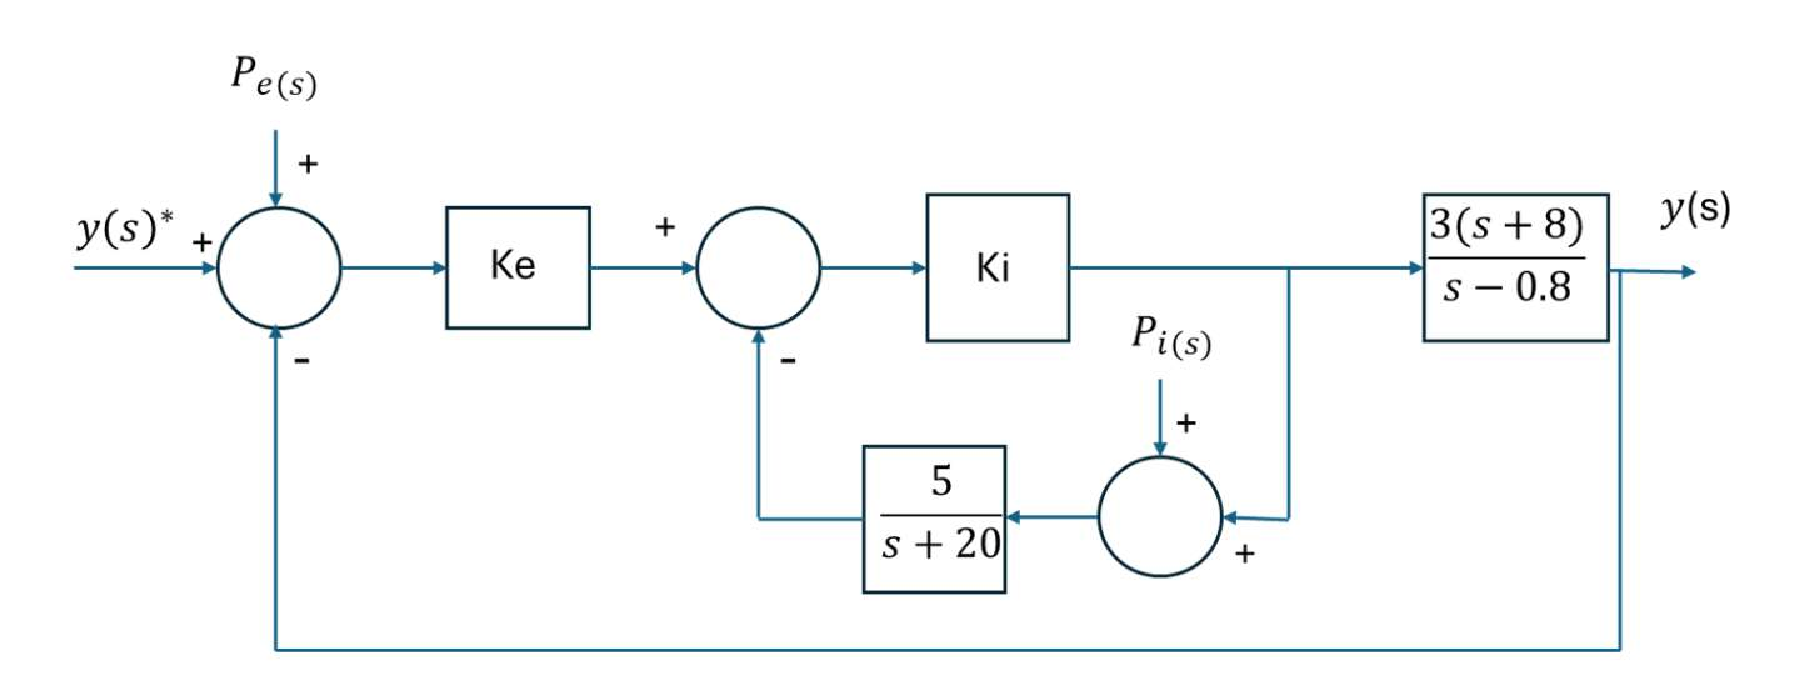
\includegraphics[width=0.7\textwidth]{Control_P2}
        \end{figure}
        \begin{enumerate}
            \item[(1)] Utilizando \(K_i = 2\), se debe diseñar el lazo externo. Elija un coeficiente de amortiguamiento adecuado y, utilizando LGR, encuentre el controlador proporcional necesario para obtener una frecuencia natural de \(\omega_n = 3.5 \, \text{rad/seg}\). (10/50)
            \item[(2)] Existen dos perturbaciones en el sistema, \(P_e(s)\) y \(P_i(s)\). ¿Cuál de estas perturbaciones tiene mayor probabilidad de producir inestabilidad asintótica en el sistema de lazos anidados? Fundamente su respuesta. (10/50)
            \item[(3)] Por envejecimiento, la ganancia \(K_i\) disminuye a un décimo del valor original. El sistema diseñado en b.1 ¿sigue siendo asintóticamente estable en ese caso? Fundamente su respuesta. (10/50)
        \end{enumerate}
    \end{itemize}
    
%------------------------
\begin{solution}
\subsection*{a)-1)}
Primero se dibuja el LGR de la planta
%----LGR-------

Luego los puntos de arranque vienen dados:
\begin{align}
    1+K(s)G(s) &= 0\\
    K(s) = \frac{-(s^{2}-7s+12)}{(s+6)}
\end{align}
Luego aplicando la derivada tenemos que:
\begin{align}
    \frac{\partial K(s)}{\partial s}_{s=\sigma} = \frac{-(2s+7)(s+6)+s^{2}-7s+12}{(s+6)^{2}}=0\\
    s_{1,2} = -6 \pm 9.5
\end{align}
Luego una primera forma para obtener la ganancia critica viene dada por s=jw, es decir en el corte, por tanto:
\begin{align}
    1+ \frac{k(s+6)}{(s-3)(s-4)}&=0\\
    s^{2}-7s +12 +k(s+6)=0\\
    (jw)^{2} -7(jw) + 12 + k(jw+6) =0\\
    -w^{2} +12 +6k + j(kw-7w) =0
\end{align}
Con lo que igualando tanto parte real como compleja a 0, tenemos que:
\begin{align}
    w &= \pm 7-3485\\
    k &= 7
\end{align}
Luego para valores de k<7 el sistema es inestable. De igual manera se puede hacer por R-H, por lo tanto:
\begin{align}
    s^{2} -7s +12 + k(s+6) &=0\\
    s^{2} s(k+7) +6k+12 &= 0
\end{align} 
Luego se tiene que la tabla viene dada por:
\begin{center}
    \begin{tabular}{|c|cc|}
        \hline
        $s^{2}$ & 1 & 6k+12\\
        $s^{1}$ & k-7 & 0\\
        $s^{0}$ & 6k+12 & 0\\
        \hline
    \end{tabular}
\end{center}
Con lo que impeniendo la condiciones estabilidad tenemos que:
\begin{align}
    k-7 > 0    \Rightarrow& k>7 \\
    6k+12 > 0  \Rightarrow& k>-2
\end{align}
Luego tenemos que para k>7 el sistema es estable.
\subsection*{1) -b)}
Luego dado que el punto de llegada esta ubicado en -15.5, luego los polos ubicados en ese punto tendran la frecuencia maxima, por lo tanto tenemos que su ganancia vendra dado por:
\begin{align}
    K= \frac{\Pi \text{Distancia polos}}{\Pi \text{Distancia ceros}} = \frac{(15.5+3)(15.5+4)}{15.5-6} = 37.974
\end{align}
De manera grafica se tiene que:
%----AGREGAR LA FORMA VISUAL--------
\subsection*{2) - a)}
Luego tenemos el siguiente para el lazo externo:
%----------AGREGAR Gint-------
\begin{align}
    G_{int}(s) = \frac{K_{i}}{1+\frac{5K_i}{s+20}}= \frac{2(s+20)}{s+30}
\end{align}
Luego aplicando el teorema de valor final a una entrada escalon tenemos que:
\begin{align}
    lim_{s \rightarrow 0}\left(\frac{s \cdot \frac{1}{s}}{1+ \frac{5K_i}{(s+20)}}\right)
\end{align}
\end{solution}
%-----------------------
\question Encuentre los cortes al eje imaginario de la planta:
\begin{align}
    H(s)G(s) = \frac{(s+3)}{s^{2}-s-2}
\end{align}
%%%%%%%%%%%%%%%%%%%%%%%%%%%
\begin{solution}
\subsection*{Resolucion 3.1 (Forma 1)}
Dada la funcion de transferencia de la planta,
\begin{align}
    H(s)G(s) &= \frac{(s+3)}{s^{2}-s-2}\\
             &= \frac{(s+3)}{(s-2)(s+1)}
\end{align}
Con lo que tenemos que los polos de la planta vendran dados por $p_{1} = 2$ y $p_{2} = -1$ y el cero $z_{1} = -3$. Se debe analizar el corte con el eje imaginario, para lo cual se considera el criterio de Routh-Hurwitz,el cual nos permite analizar los rangos de ganancia que permiten la estabilidad del sistema en base a una tabla y los cambios de signos de la misma.Para esto se debe expresar la funcion de transferencia de lazo cerrado en forma polinomica, con lo que se obtiene:
\begin{align}
    1+kG(s)H(s) &= 0\\
    1+k\frac{(s+3)}{(s-2)(s+1)} &= 0\\
    (s-2)(s+1)+k(s+3) &= 0\\
    s^{2}-s-2+ks+3k &= 0\\
    s^{2}+(k-1)s-2+3k &= 0
\end{align}
Luego utilizamos la tabla tal que:
\begin{center}
    \begin{tabular}{|c|cc|}
        \hline
        $s^{2}$ & 1 & -2+3k\\
        $s^{1}$ & k-1 & 0\\
        $s^{0}$ & $\alpha_{1}$ & $\alpha_{2}$\\
        \hline
    \end{tabular}
\end{center}
Donde para obtener los valores de $\alpha_{1}$ y $\alpha_{2}$ se utilizan las formulas asociadas:
\begin{align}
    \alpha_{1} &= \frac{(3k-2)(k-1)-0}{k-1} = (3k-2)\\
    \alpha_{2} &= 0
\end{align}
(Yo suelo utilizar este ayuda memoria para no olvidarme)
\begin{center}
    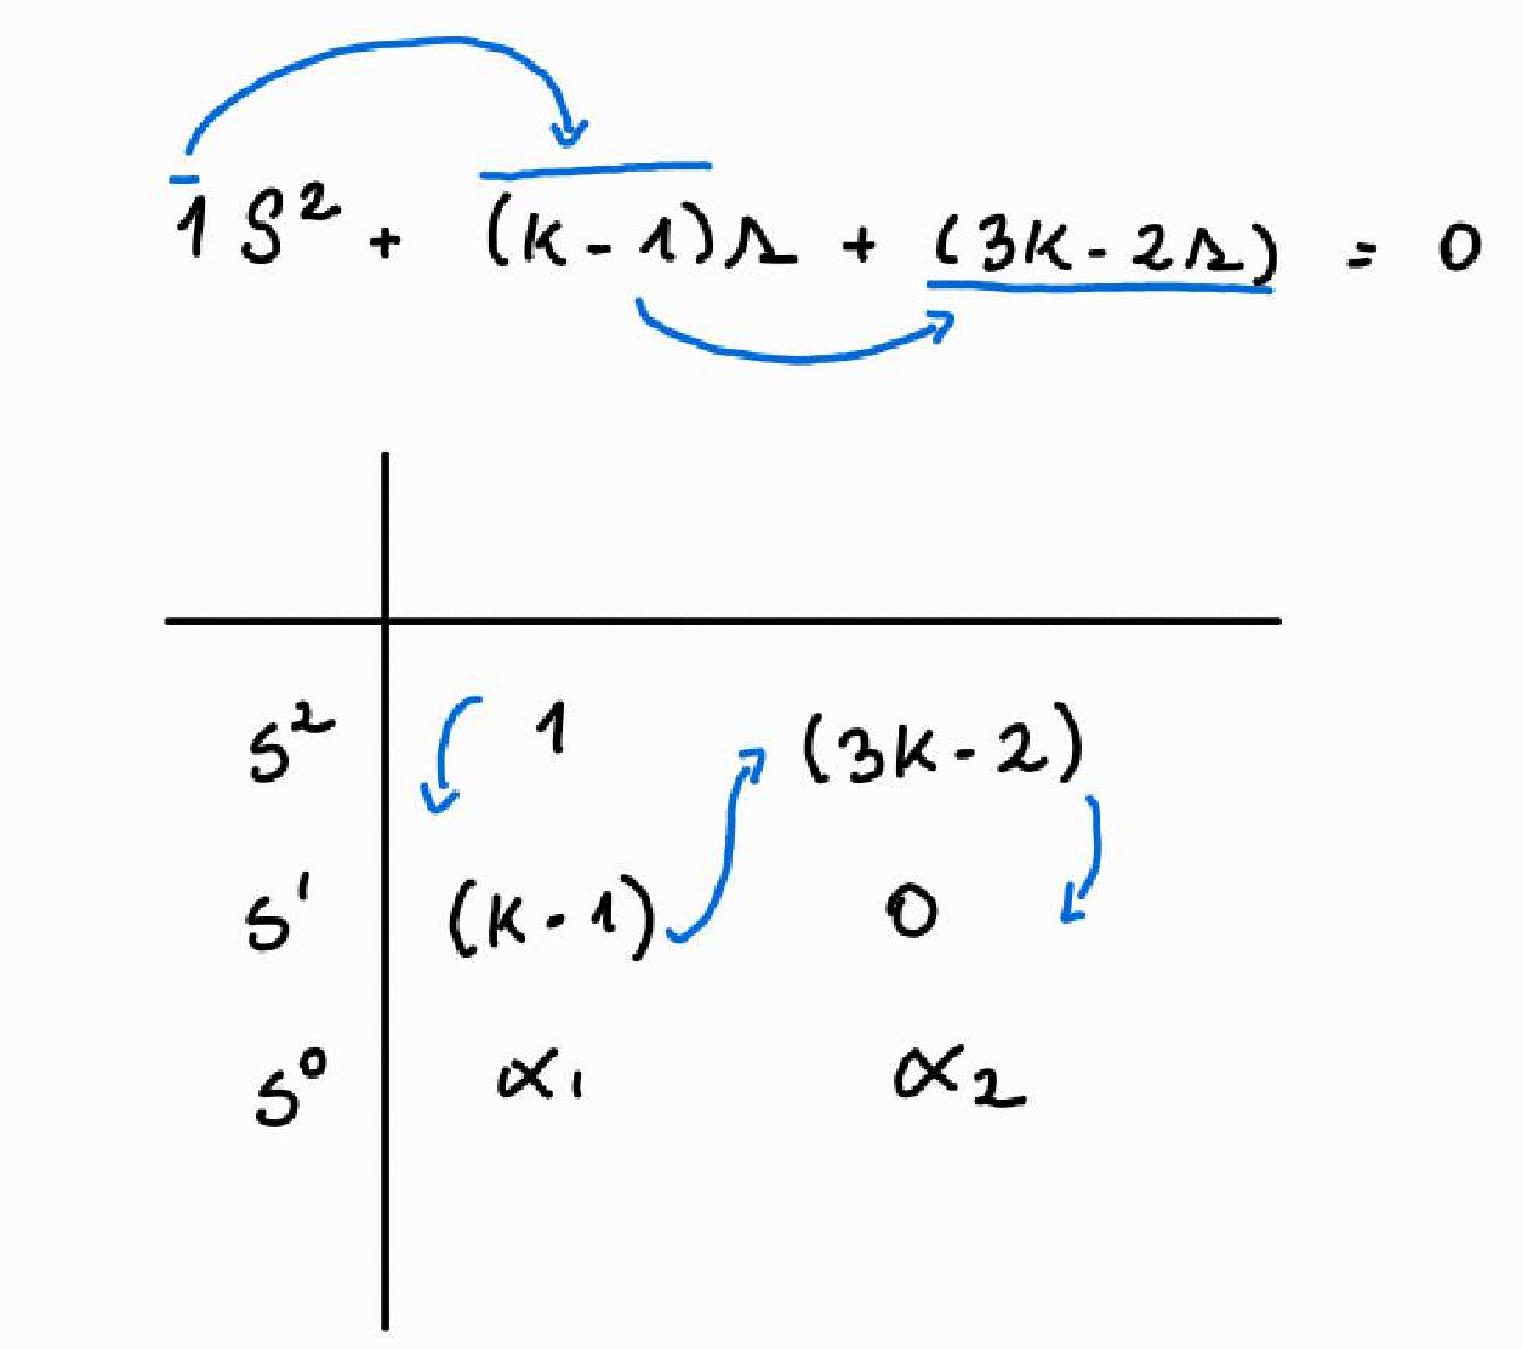
\includegraphics[width=0.3\textwidth]{Auxiliar_2_8}
    \captionof{figure}{La idea es situar en la columna de la izquierda el mayor de grado hasta el menor grado, posteriormente reconocemos los coeficientes del polinomio y trazamos las flechas azules, desde la esquina superior izquierda bajando y luego subiendo hasta completar todo los coeficientes del polinomio (En caso de no haber se rellena con 0).}
  \end{center}
  \begin{center}
    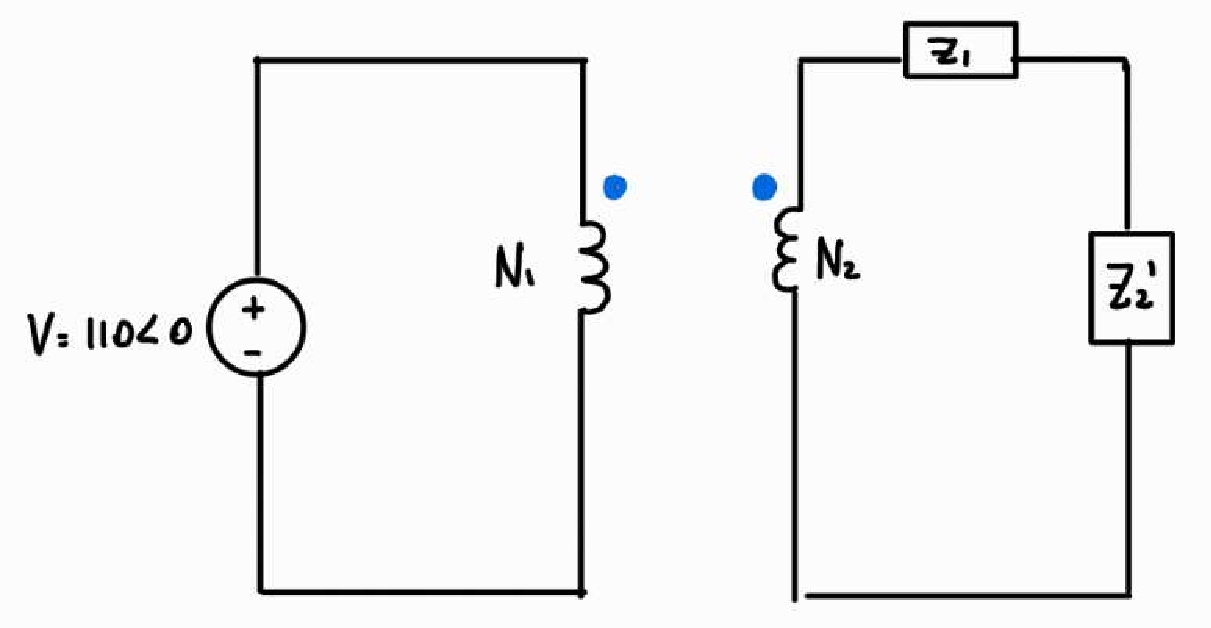
\includegraphics[width=0.55\textwidth]{Auxiliar_2_9}
    \captionof{figure}{Una vez ubicados los coeficientes se deben calcular los coeficientes, por lo que por ejemplo para calcular $\alpha_{1}$ se utiliza el termino superior y se realiza un \textit{Pivote} y luego se realizan las multiplicaciones diagonales y se restan y se dividen por el \textit{Pivote}.}
  \end{center}
  \begin{center}
    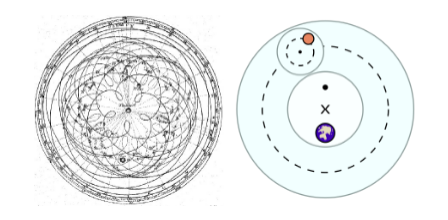
\includegraphics[width=0.55\textwidth]{Auxiliar_2_10}
    \captionof{figure}{Para $\alpha_{2}$ se utiliza el mismo procedimiento}
  \end{center}
Esta metodologia utilizaba para no olvidarme, pero siempre es a criterio personal.Luego tenemos que la matriz vendra dada por:
\begin{center}
    \begin{tabular}{|c|cc|}
        \hline
        $s^{2}$ & 1 & 3k-2\\
        $s^{1}$ & k-1 & 0\\
        $s^{0}$ & $3k-2$ & 0\\
        \hline
    \end{tabular}
\end{center}
El criterio de Routh-width se basa en analizar la segunda columna, para la cual el cambio de signo es equivalente a entrar a zona donde este sea inestable, o equivalentemente cruze el semiplano derecho, por lo que se debera cumplir que en todo momento la primera columna sea positiva, por lo que se obtiene un intervalo vendra dado por (Es importante destacar que este analisis se realiza considerando que $k>0$):
\begin{align}
    k-1 &> 0\\
    3k-2 &> 0
\end{align}
Con lo que se debe cumplir en simultaneo que $k>1$ y $k>\frac{2}{3}$, por lo que se obtiene que $k>1$ cumplira ambas condiciones que permitira la estabilidad .Finalmente se obtiene que el corte con el eje imaginario vendra dado por los momentos en que existe cambio de signo, por lo que estos correpsonden a $k_{1} = \frac{2}{3}$ y $k_{2}=1$, con lo que reemplazando sobre la funcion de transferencia de los polos de lazo cerrado se obtiene que:
\subsubsection*{Caso 1: $K=\frac{2}{3}$}
\begin{align}
    s^{2}+(k-1)s-2+3k &= 0\\
    (jw)^{2}+(k-1)jw-2+3\cdot \left|\frac{2}{3}\right| &= 0\\
    -w^{2}+jw\frac{-1}{3} +0 &= 0\\
\end{align}
Luego igualamos separamos parte real e imaginaria y obtenemos que:
\begin{align}
    -w^{2} &= 0\\
    -\frac{1}{3}w &= 0
\end{align}
Con lo que se obtiene que $s=0$, por lo que el corte se obtiene en el origen.
\subsubsection*{Caso 2: K=1}
Analogamente tenemos que:
\begin{align}
    s^{2}+(k-1)s-2+3k &= 0\\
    (jw)^{2}+(k-1)jw-2+3\cdot 1 &= 0\\
    -w^{2}+jw(1-1) -2+3 &= 0\\
\end{align}
Luego tenemos solo parte real,:
\begin{align}
    w^{2} &= \pm 1
\end{align}
De esta manera tenemos que los cortes se cumplen para $s= \pm j$.
\subsection*{Resolucion 3.2 (Forma 2)} 
Otra condicion que se utilizara con mucha mas frecuencia es a la condicion de angulo , la cual vendra dada por:
\begin{align}
    \angle \sum \Theta_{polos} - \sum \Theta_{ceros} = \pm 180^{\circ} + n360^{\circ} 
\end{align}
De esta manera tenemos que encontrar los angulos asociados a los polos y ceros deberan cumplir tal condicion, pero ademas deberemos considerar que s=jw , dado nos interesa el corte en el eje real que cumpla dicha condicion de angulo.Retomando la funcion de transferencia:
\begin{align}
    H(s)G(s) &= \frac{(s+3)}{s^{2}-s-2}\\
             &= \frac{(s+3)}{(s-2)(s+1)}
\end{align}
Tenemos luego que existe $p_{1}=-1$,$p_{2}=2$ y $z_{1}=-3$ , con lo que luego tenemos que se debe cumplir que:
\begin{align}
    \theta_{z_{1}} - (\theta_{p_{1}} + \theta_{p_{2}}) &= 180
\end{align}
Que graficamente correspondera a lo siguiente (Debemos recordar siempre como es la apertura de los angulos):
\begin{center}
    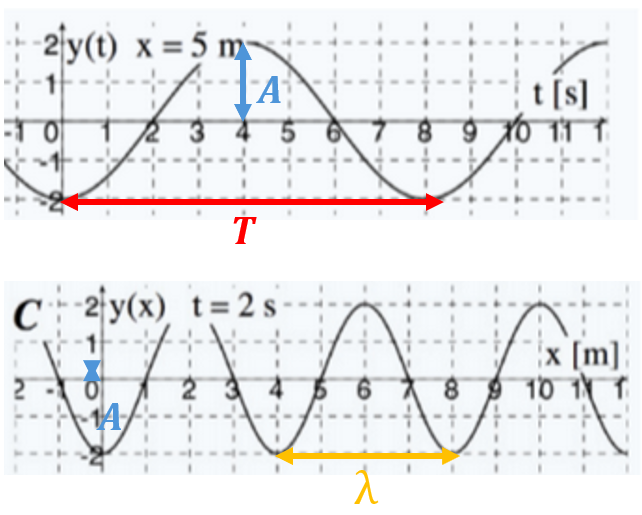
\includegraphics[width=0.55\textwidth]{Auxiliar_2_13}
    \captionof{figure}{Recordatorio de como se miden los angulos para algun punto que pertenece al LGR}
  \end{center}
  \begin{center}
    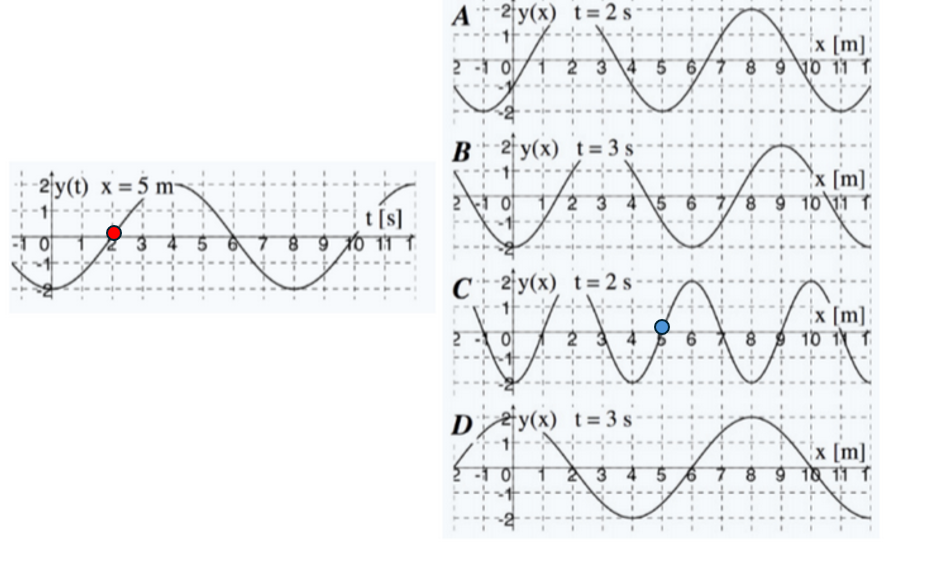
\includegraphics[width=0.55\textwidth]{Auxiliar_2_12}
    \captionof{figure}{Angulos para la funcion de transferencia vista con anterioridad} 
  \end{center}
\begin{align}
    tan(\theta_{p_{1}})&= \frac{w}{1}\\
    tan(\theta_{p_{2}})&= \frac{w}{2}\\
    tan(\theta_{z_{1}})&= \frac{w}{3}
\end{align}
Con lo que sus respectivos angulos corresponderan a:
\begin{align}
    \theta_{p_{1}} &= atan(\frac{w}{1})\\
    \theta_{p_{2}} &= 180 - atan(\frac{w}{2})\\
    \theta_{z_{1}} &= atan(\frac{w}{1})
\end{align}
Con lo que reemplazando en la condicion de angulo se obtiene que:
\begin{align}
    atan(\frac{w}{3}) - (atan(\frac{w}{1}) + 180 - atan(\frac{w}{2})) &= 180\\
    atan(\frac{w}{3}) - atan(\frac{w}{1}) - 180 + atan(\frac{w}{2}) &= 180\\
    atan(\frac{w}{3}) - atan(\frac{w}{1}) + atan(\frac{w}{2}) &= 360
\end{align}
Donde ademas sabemos que 360 es equivalente a 0, por lo que se obtiene que:
\begin{align}
    atan(\frac{w}{3}) - atan(\frac{w}{1}) + atan(\frac{w}{2}) &= 0
\end{align}
Luego queda por resolver la ecuacion , la cual entrega tres soluciones:
\begin{align}
    w_{1} &= 0\\
    w_{2} &= +j\\
    w_{3} &= -j
\end{align}
Mismas obtenidas con anterioridad.
\end{solution}

\end{questions}
\newpage
%%%%%%%%%%%%%%%%%%%%%%%%%%%

\end{document}